\section{Wellen}
\subsection{Definition}
\paragraph{Beispiele:} Elektromagnetische Wellen (Radio, Licht...), Schallwelle, Wasserwelle, Erdbebenwelle... 

\paragraph{Welle:} 
Ein sich räumlich fortpflanzender Bewegungszustand, der \underline{Energie}, aber \underline{keine Materie} transportiert.

\paragraph{Wellenausbreitung im Medium:}
Jeder Oszillator ist an seine Nachbarn gekoppelt und wird zu einer erzwungenen Schwingung angeregt.

\vspace{2mm}
\underline{Skizze}\\
Das 3. Teilchen beschleunigt das 4. Teilchen und erfährt die reactio. Die Ausbreitung erfolgt umso schneller, je größer D und je kleiner m ist ($a = \dfrac{F}{m}$)

\subsection{Wichtige physikalische Größen}
Während ein einzelner Oszillator eine Schwingung (mit der Periodendauer T) vollführt, ist die Welle gerade eine Wellenlänge $\lambda$ weiter vorgerückt. \\
Also beträgt die Ausbreitungsgeschwindigkeit c der Welle
\vspace{2mm} \\
$ c = \dfrac{\lambda}{T} = \lambda \ast f $

\vspace{2mm}
Die Geschwindigkeit jedes einzelnen Oszillators v bei der erzwungenen Schwingung wird - zur Unterscheidung von der Ausbreitungsgeschwindigkeit c - ab jetzt mit \underline{Schnelle v} bezeichnet.
\vspace{2mm} \\
\paragraph{Transversalwelle:} 
Bei einer Transversalwelle steht der Schwingungsvektor \underline{senkrecht} zur Ausbreitungsrichtung. Wellenberge und Wellentäler laufen über den Wellenträger. \\
Bsp.: elektromagnetische Wellen, S-Wellen beim Erdbeben. \\
\underline{Mechanische} Transversalwellen können nur entstehen, wenn zwischen den Oszillatoren \underline{elastische Querkräfte} wirksam sind (also nur im Festkörper).

\paragraph{Longitudinalwelle:} 
Bei einer Longitudinalwelle steht der Schwingungsvektor \underline{parallel} zur Ausbreitungsrichtung. \underline{Verdichtungen} und \underline{Verdünnungen} laufen über den Wellenträger. \\
Bsp.: Schallwellen, Wasserwellen, P-Wellen beim Erdbeben. \\
Longitudinalwellen können dann entstehen, wenn zwischen den Oszillatoren Kräfte wirksam sind, die der Volumenänderung entgegenwirken.\\
\underline{Mechanische} Longitudinalwellen sind "Druckwellen" (existieren in Festkörper, Flüssigkeiten und Gasen) \\
Zur Skizze: $\overrightarrow{v} \perp \overrightarrow{c}$ \\
Zur Skizze 2: $\overrightarrow{v} \parallel \overrightarrow{c}$ \\
\underline{Skizzen RS zu AB10.04. } \\
Die Ausbreitungsgeschwindigkeit c wird auch \underline{Phasen}geschwindigkeit ($v_{ph}$) genannt, weil sie die Geschwindigkeit ist, mit der sich eine bestimmte Phasenlage der Oszillation über den Wellenträger ausbreitet.

\subsection{Zeitliche und räumliche Darstellung einer Welle}
\underline{Zeichnung zeitl, Darstellung RS zu AB10.04. }
\vspace{2mm} \\
Beim "zeitlichen Durchblick" ist der zeitliche Verlauf der erzwungenen Schwingung an einem Ort dargestellt. \\
Beim "räumlichen Durchblick" zu einem Zeitpunkt t stellt sich die Welle dar, wie man sie zu diesem Zeitpunkt im Raum sieht (Fotografie). Der Oszillator am Kopf der Welle beginnt gerade zu diesem Zeitpunkt seine Schwingung, sein Nachbaroszillator schwingt bereits einen kurzen Moment, dessen Nachbaroszillator schwingt noch einen Moment länger etc. Man sieht alle Phasenzustände nebeneinandergelegt. \\
Beim "diagonalen Durchblick" verfolgt man eine bestimmte Schwingungsphase (Zum Beispiel den Kopf der Welle oder den ersten Wellenberg) bei seiner Wanderung über den Wellenträger.

\subsection{Die Bewegungsgleichung einer Welle}
1. Der Oszillator am Punkt x=0, der zum Zeitpunkt t=0s von der Welle erfasst wird, hat die Bewegungsgleichung $ s_{(0cm, t)} = \hat{s} \ast sin(\omega \ast t) $ 
\vspace{2mm} \\
2. Der Oszillator am Punkt x, der zum Zeitpunkt $ t = \frac{x}{c} $ von der Welle erfasst wird, hat die Bewegungsgleichung $ s_{(x, t)} = \hat{s} \ast sin(\omega \ast t - \dfrac{2 \pi}{T} \ast \dfrac{x}{c})  = \hat{s} \ast sin(\omega \ast (t - \dfrac{x}{c})) $ 
\vspace{3mm} \\
$ s_{(x,t)} $ ist eine "doppelt-periodische" Funktion. Für konstantes x ist die Periode die Schwingungsdauer T, für konstantes t ist die Periode die Wellenlänge $\lambda$. 
\vspace{2mm} \\
Die Bewegungsgleichung ist die Lösungsfunktion der Differentialgleichung der Welle: \\ $ F_{(x,t)} = m \ast \ddot{s}_{(x,t)} $ \\
Die Kraft auf einen Oszillator ist proportional zur Krümmung der Kurve $ s_{(x,t)} $ 
\vspace{2mm} \\
$ F_{(x,t)} = D \ast s''_{\hspace{1,5mm}(x,t)} $ 
\vspace{2mm} \\
$ D \ast s''_{\hspace{1,5mm}(x,t)} = m \ast \ddot{s}_{(x,t)} $	
\vspace{2mm} \\
Kontrolle: Einsetzen von $s_{(x,t)} = \hat{s} \ast sin(\omega \ast t - \frac{2\pi}{\lambda} \ast x) $
\vspace{3mm} \\
$ D \ast (-\hat{s} \ast (\frac{2\pi}{\lambda})^{2} \ast sin(\omega \ast t - \frac{2\pi}{\lambda} \ast x)) = m \ast (-\hat{s} \ast \omega^{2} \ast sin(\omega \ast t - \frac{2\pi}{\lambda} \ast x)) $
\vspace{2mm} \\
$ D \ast (\frac{2\pi}{\lambda})^{2} = m \ast \omega^{2} $ 
\vspace{2mm} \\
$ D \ast (\frac{2\pi}{\lambda})^{2} = m \ast (\frac{2\pi}{\lambda})^{2} $
\vspace{2mm} \\
$ D \ast \frac{1}{\lambda{2}} = m \ast \frac{1}{T^{2}} $
\vspace{2mm} \\
$ \frac{D}{m} = \frac{\lambda{2}}{T^{2}} = c^{2} $
\vspace{2mm} \\
$ c = \sqrt{\frac{D}{m}} $	

\paragraph{Zeigerdarstellung:} Jedem Oszillator am Ort x kann ein Zeiger zugeordnet werden, der gegen den Uhrzeigersinn rotiert und dessen y-Komponente die momentane Elongation $s_{(x,t)}$ angibt. 

\newpage

\subsection{Einschub: Überlagerung zweier harmonischer Schwingungen an einem Ort}
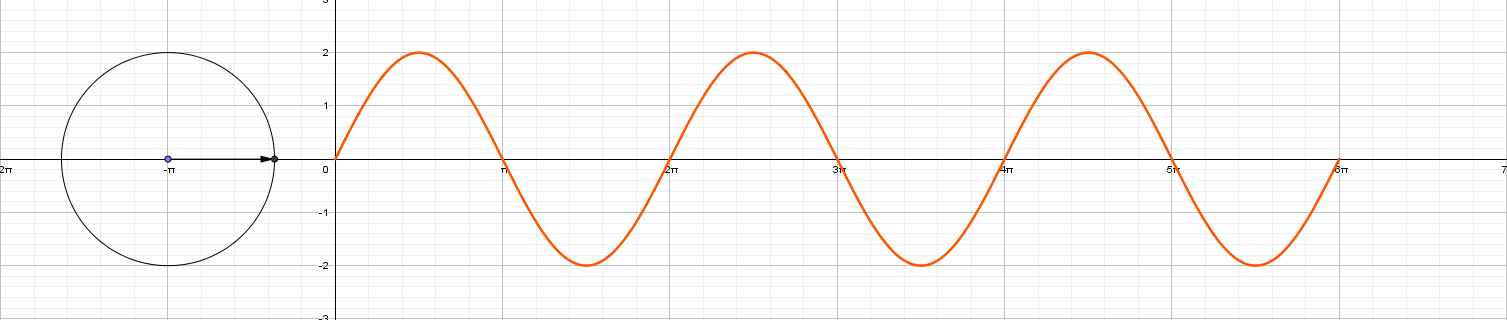
\includegraphics[scale=0.426]{sin6_1}
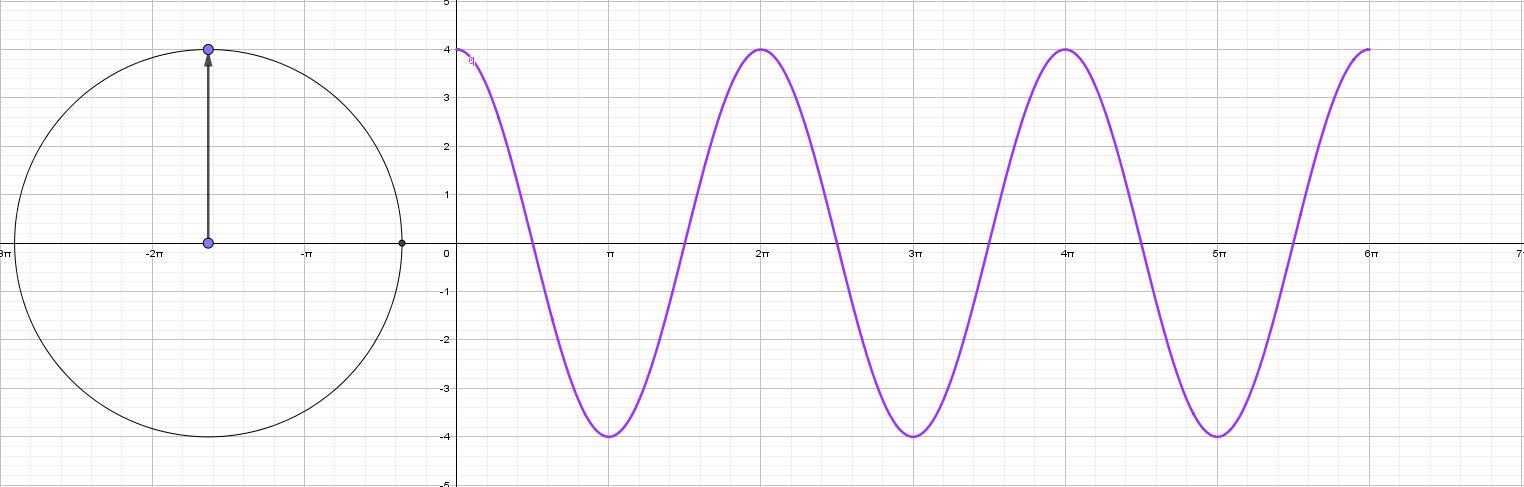
\includegraphics[scale=0.421]{sin6_2}
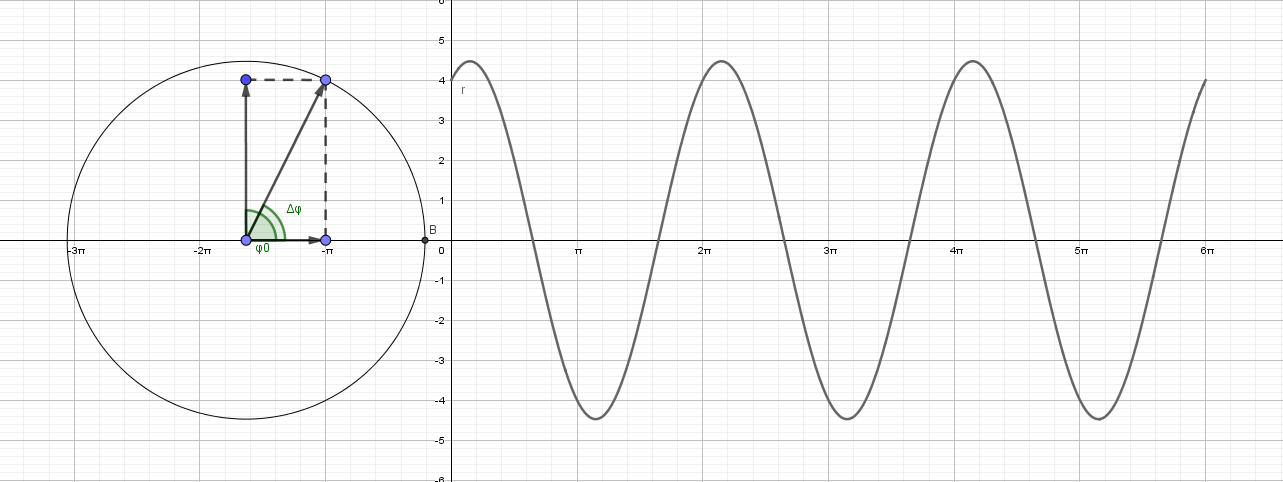
\includegraphics[scale=0.5]{sin6_3}
\vspace{2mm} \\
Die Zeiger von $s_{1}$ und $s_{2}$ rotieren mit der gleichen Winkelgeschwindigkeit $\omega$ gegen den Uhrzeigersinn. Ihre relative Lage zueinander bleibt dabei immer gleich. Das Zeigerdiagramm ermöglicht es uns, durch die vektorielle Addition der Zeiger von $s_{1}$ und $s_{2}$ den resultierenden Zeiger $s_{res}$zu bestimmen. Die Länge des resultierenden Zeigers entspricht $\hat{s}_{res}$, die Phasendifferenz $\Delta \varphi$ bezüglich z.B. $s_{1}$ gibt an, um welche Phase der Schwingung $s_{res}$ gegenüber $s_{1}$ vorauseilt. Zudem erhält man die aktuelle Phasenlage des Zeigers für den Zeitpunkt, den das Zeigerdiagramm darstellt. 
\newpage

\subsection{Überlagerung von Wellen - Allgemeines Prinzip}
\paragraph{Prinzip der ungestörten Überlagerung von Wellen:}
Treffen an einer Stelle eines Wellenträgers mehrere Wellen aufeinander, so addieren sich dort die Elongationen und Schnellen der Schwingungen. Nach dem Zusammentreffen laufen die Wellen ungestört weiter. \\
Die ungestörte Überlagerung mehrerer Wellen von gleicher Frequenz (gleicher Wellenlänge) wird als Interferenz bezeichnet.

\subsection{Interferenz}
\subsubsection{Überlagerung gleich laufender Wellen}
Bei Interferenz zweier Wellen gleicher Frequenz ergibt sich \\
1. konstruktive Interferenz (maximale Verstärkung) bei einer Phasendifferenz von $\Delta \varphi = 0$ oder $\Delta \varphi = k \ast 2 \pi $, entsprechend einem Gangunterschied von $ \delta = 0 $ oder $ \delta = k \ast \lambda $ mit k = 1,2,3,... $(k \in \mathbb{N})$ \\
2. destruktive Interferenz (maximale Abschwächung) bei einer Phasendifferenz von $ \Delta \varphi = (2k-1) \ast \frac{\lambda}{2} $ mit k = 1,2,3,... $(k \in \mathbb{N})$ \\

\subsubsection{Überlagerung gegenlaufender Wellen}
Bei der Überlagerung gleicher, gegenlaufender Wellen ergeben sich \underline{stehende} Wellen:
\vspace{1mm} \\
\begin{itemize}
	\item Es gibt Stellen, an denen die Amplitude stets 0 ist. Sie heißen Schwingungsknoten. \\
	\item Es gibt Stellen mit stets maximaler Amplitude ($\hat{s}_{res} = \hat{s_{1}} + \hat{s_{2}} $). Sie heißen Schwingungsbäuche. \\
	\item Die Oszillatoren schwingen zwischen zwei Knoten phasengleich, aber mit unterschiedlicher Amplitude. Vor und nach einem Knoten schwingen sie gegenphasig. \\
	\item Die Entfernung zwischen benachbarten Knoten beträgt $\frac{\lambda}{2}$, ebenso zwischen benachbarten Bäuchen.
\end{itemize}
Auf gelbem Blatt 3/12 T
\vspace{2mm} \\
Zum Zeitpunkt, an dem die Oszillatoren die Ruhelage passieren, erreichen sie ihre maximale Schnelle. Diese ist unterschiedlich. Die Gesamtenergie liegt also als kinetische Energie vor ($W_{ges} = \frac{1}{2} \ast m \ast \hat{v}^{2} $). Zum Zeitpunkt, an dem alle Oszillatoren ihre maximale Elongation erreichen, sind alle Oszillatoren in Ruhe. Ihre Beschleunigung ist maximal. Die Gesamtenergie liegt als potenzielle Energie vor ($W_{ges} = \frac{1}{2} \ast D \ast \hat{s}^{2}$). \\
Allgemein: Die stehende Welle transportiert keine Energie. An den Knoten besitzen die Oszillatoren keine Energie, an den Bäuchen besitzen die Oszillatoren maximale Energie. 
\vspace{5mm} \\

\textbf{Überlagerung auf der Verbindungsgerade zweier Wellenzentren:}
\vspace{2mm} \\
1. Für die Schwingungsbäuche $ \delta = k \ast \lambda $; $ k \in \mathbb{N}_{0} $
\vspace{1mm} \\
$ 2 \ast x = k \ast \lambda $
\vspace{1mm} \\
$ x = k \ast \frac{\lambda}{2} $
\vspace{3mm} \\
2. Für die Schwingungsknoten $ \delta = (2k -1) \ast \frac{\lambda}{2} $ ; $ k \in \mathbb{N}$
\vspace{1mm} \\
$ 2 \ast x = (2k-1) \ast \frac{\lambda}{2} $
\vspace{1mm} \\
$ x = (2k-1) \ast \lambda $

\subsection{Reflexion mechanischer Wellen}
Am festen Ende werden aufgrund von Actio-Reactio Elongation und Schnelle umgekehrt (Phasensprung um $\pi$) \\
Am losen Ende werden Elongation und Schnelle ohne Phasensprung reflektiert.
\vspace{5mm}\\

Bei Longitudinalwellen gelten die selben Gesetzmäßigkeiten bei der Reflexion wie bei Transversalwellen: \\
Am festen Ende werden Elongation und Schnelle umgekehrt (Phasensprung um $\pi$), am losen Ende behalten sie ihre Richtung bei. 
\vspace{2mm} \\
Zu AB08.06 Aufgabe 1: Die Welle reflektiert am rechten Ende und überlagert sich mit der einlaufenden Welle. Da im Bereich zwischen 6m und 8m eine doppelt so große Amplitude erscheint und am rechten Ende die Auslenkung 0 beträgt, ist das rechte Ende fest. Die Welle hat zu diesem Zeitpunkt insgesamt 10m zurückgelegt. 
\vspace{2mm} \\
Aufgabe 2: $ c = \frac{x}{t} = \frac{10m}{2,5s} = 4 \frac{m}{s} $ 
\vspace{1mm} \\
Die Welle wäre ohne Reflexion in t=3s die Strecke $ x = c \ast t = 12m $ weit gekommen.

\subsection{Eigenschwingungen auf begrenztem Wellenträger}
Auf einem begrenzten Wellenträger können sich nur bei bestimmten Anregungsfrequenzen, den sogenannten Eigenfrequenzen des Wellenträgers, stehende Wellen ausbilden. Er zeigt dann ein typisches Resonanzverhalten (Das heißt die Schwingungsamplitude kann ein vielfaches der Erregerschwingungsamplitude betragen). Die Eigenschwingungen heißen k-te Harmonische ($k \in \mathbb{N}$). 
\vspace{2mm} \\
Randbedingungen:
\begin{itemize}
	\item Zwei gleiche Enden: 
	\subitem $ \lambda_{k} = \frac{2 \ast l}{k} = \frac{\lambda_{1}}{k} , (k \in \mathbb{N}) $
	\subitem $ f_{k} = k \ast \frac{c}{2 \ast l} = k \ast \frac{c}{\lambda_{1}} = k \ast f_{1} ,  (k \in \mathbb{N}) $
	
	\item Zwei ungleiche Enden:
	\subitem $ \lambda_{k} = \frac{4 \ast l}{(2k-1)} = \frac{1}{(2k-1)} \ast \lambda_{1} , (k \in \mathbb{N}) $
	\subitem $ f_{k} = (2k-1) \ast \frac{c}{4 \ast l} = (2k-1) \ast f_{1} , (k \in \mathbb{N}) $ 
\end{itemize}